% !TEX encoding = UTF-8
%Koma article
\documentclass[fontsize=12pt,paper=letter,twoside]{scrartcl}

%Standard Pre-amble
\usepackage[top=4cm,bottom=4cm,left=3cm,right=3cm,asymmetric]{geometry}
%\geometry{landscape}                % Activate for for rotated page geometry
%\usepackage[parfill]{parskip}    % Begin paragraphs with an empty line rather than an indent
\usepackage[table,xcdraw]{xcolor}
\usepackage{graphicx}

\usepackage{amsmath}
\usepackage{amssymb}
\usepackage{epstopdf}
\DeclareGraphicsRule{.tif}{png}{.png}{`convert #1 `dirname #1`/`basename #1 .tif`.png}
% Listings needs package courier
\usepackage{listings} % Needs 
\usepackage{courier}

\usepackage[framemethod=TikZ]{mdframed}
\usepackage{url}

\usepackage{sty/bsymb} %% Event-B symbols
\usepackage{sty/eventB} %% REQ and ENV
\usepackage{sty/calculation}

%Maths
\usepackage{amssymb,amsmath}
\def\Fl{\mathbb{F}}
\def\Rl{\mathbb{R}}
\def\Nl{\mathbb{N}}
\def\Bl{\mathbb{B}}
\def\St{\mathbb{S}}
\newcommand{\ovr}{\upharpoonright}
\newcommand{\var}[1]{\textit{#1}}
%Useful definitions
\newcommand{\mv}[1]{\textit{m\_#1}}
\newcommand{\cv}[1]{\textit{c\_#1}}
\newcommand{\degree}[1]{^{\circ}\mathrm{#1}}
%\newcommand{\comment}[1]{{\footnotesize \quad\texttt{--}\textrm{#1}}}
\newcommand{\im}[1]{i\texttt{-\!#1}}

\usepackage[headsepline]{scrpage2}
\pagestyle{scrheadings}
\ihead[]{\small EECS4312 Report1}
\ohead[]{\small \thepage}
\cfoot[]{}
\ofoot[]{}


%%%%PVS environment%%%%%%%%%%%%%%%%%%%
\lstnewenvironment{pvs}[1][]
    {\lstset{#1,captionpos=b,language=pvs,
    mathescape=true,
    basicstyle=\small\ttfamily,
    numbers=none,
    frame=single,
    % numberstyle=\tiny\color{gray},
    % backgroundcolor=\color{lightgray},
    firstnumber=auto
    }}
    {}
 %%%%%%%%%%%%%%%%%%%%%%%%%%%%%%%%
 
%%%%Verbatim environment%%%%%%%%%%%%%%%%%%%
\lstnewenvironment{code}[1][]
    {\lstset{#1,captionpos=b,
    mathescape=true,
    basicstyle=\small\ttfamily,
    numbers=none,
    frame=single,
    % numberstyle=\tiny\color{gray},
    % backgroundcolor=\color{lightgray},
    firstnumber=auto
    }}
    {}

% \newenvironment{boxed}[1]
%    {\begin{center}
%    #1\\[1ex]
%    \begin{tabular}{|p{0.9\textwidth}|}
%    \hline\\
%    }
%    { 
%    \\\\\hline
%    \end{tabular} 
%    \end{center}
%    }
 %%%%%%%%%%%%%%%%%%%%%%%%%%%%%%%%
 
 %Text in a box
\newenvironment{textbox}
    {\begin{center}
    \begin{tabular}{|p{0.9\textwidth}|}
    \hline\\
    }
    { 
    \\\\\hline
    \end{tabular} 
    \end{center}
    }

\usepackage{hyperref}

%Highlight \hl{}
\usepackage{soul}

\usepackage{enumitem}
\newlist{mylist}{itemize}{1}
\setlist[mylist]{label=\textbullet,leftmargin=1cm,nosep}

\usepackage{multirow}

% Reduce space between figure and caption
%\usepackage{caption}
%\captionsetup[table]{font=small,skip=0pt}     %% Adjust here
%or equivalently 
\usepackage[font=small,skip=4pt]{caption}
% Set the header
\ihead[]{\small Isolette Specification: EECS4312 Assignment}
\title{Isolette Specification:\\ EECS4312 Assignment}


\date{\today} % Display a given date or no date

\begin{document}
\maketitle

\begin{abstract}
As stated in the course outline, you are required to read parts of  the Handbook \cite{REMH}  each week. In this assignment you will be constructing the function table for the Isolette described in \cite{REMH} (Appendix A). 

The Handbook omits E/R-descriptions and function  tables. Hence, the main learning outcomes for this Assignment is to complete a precise requirements document for the Isolette by providing the E/R-descriptions and function tables. You must check the function tables with PVS for completeness, disjointness and safety.

\textbf{What you must do}:

\begin{mylist}
\item Read this document and the  specification of the Isolette (in Appendix A of \cite{REMH}). We will be using only part of this Isolette requirements document \cite{REMH}. Also, there are some problems in \cite{REMH} which your are required to fix in your submission.
\item Provide a precise requirements document for the Isolette by completing the LaTeX template (isolette-assign.tex) in the SVN (LaTex files provided).
\item Complete the parts in the template \hl{highlighted in yellow}. By completing the provided template you will see the overall structure of a precise requirements documents. The final document you produce is \texttt{isolette-assign.pdf}.
\item Before the due date, submit an electronic copy of \texttt{isolette-assign.pdf} and place a printed copy of the PDF in the drop box.
\item You must also submit your PVS files and proofs in a folder \texttt{pvs}: submit 4312 assign isolette
\end{mylist}

\end{abstract}

\section*{Revisions}
\small
%%%%%%%%%%%%Table of revisions%%%%%%%%
\begin{tabular}{|l|l|p{4in}|}
\hline
Date & Revision& Description \\ 
\hline
22 October  2015 
& 1.0       
& Initial specification of Assignment: Isolette system\\ 
\hline
23 October 2015 & 2.0 & Revised E/R descriptions,  Alarm Off Hysteresis and Non-circular data-flow\\
\hline
\end{tabular}
%%%%%%%%%%%%%%%%%%%%%%%%%%%%%%%%

\tableofcontents
\listoffigures
\normalsize

%%%%Rest of your document goes here%%%%%%%%%%%%%%%%%%%
\newpage
% !TEX root =  isolette-readme.tex
\section{The Isolette}

As stated in the course outline, you were required to read parts of  the Handbook \cite{REMH}  each week. In this assignment you will be constructing the function table for the Isolette described in \cite{REMH} (Appendix A). The Handbook omits E/R-descriptions and function  tables. Hence, the main learning outcomes for this Assignment are:

\begin{mylist}
\item Demonstrate that you can write E/R-descriptions.
\item Demonstrate that you can describe a complete and disjoint function table for a safety critical system (the Isolette) and that you can also derive important safety invariants that the function table must satisfy (to validate your specification).
\item The above items must be completed in the context of a LaTeX template (supplied in the SVN) with much material already present. You must complete the parts \hl{highlighted in yellow}. By completing the provided template you will see the overall structure of a precise requirements documents.
\end{mylist}

\smallskip
\noindent As stated above, you will complete a precise Requirements Document.  You will need to do further requirements elicitation from the customer (i.e. the instructor and TAs) where requirements are unclear. The answers you obtain to the elicitation questions must be recorded in the E/R-descriptions and function table (where relevant).

\section{E/R-descriptions}

\textbf{Required Readin}g: Read Section~2, Section~3, Section~6, Appendix~A and Appendix F of \emph{Get it Right the First Time: Writing Better Requirements} \cite{telelogic}---available in the SVN. A summary of some of the above information follows.

\subsection{What are requirements?}

\begin{mdframed}
Understand and agree upon what users want before attempting to create
solutions.
\end{mdframed}

Finding out what is needed instead of rushing into presumed solutions is the key
to every aspect of system development. Most technical problems can be solved,
given determination, patience, a skilled team---and a well-defined problem to
solve.

\bigskip
\begin{mdframed}
A precise requirements document will contain all the information needed by the developers to build the system wanted by the users---and no more (i.e. it should not be polluted with design and implementation detail).
\end{mdframed}


\subsection{Why do requirements?}
Writing requirements is not an end in itself. But it is also not merely extra work or an
additional activity to ensure checks and balances or to meet a standard.
Requirements have a real purpose in the development of any system.
They are essential:
\begin{mylist}
\item To show results the users want from the system.
\item  To show traceability back to sources and the history of changes.
\item  To show what the organization needs.
\item  To show what the system must do.
\item  To form a basis for the design and design optimization (without being polluted by design or implementation detail)
\item  To enable a logical approach to change management.
\item  To partition the work out to contractors.
\item  To act as a foundation for testing and payment.
\item  To test the system or any of its parts during development.
\item  To communicate the basics about the system in non-technical terms to all
participants
\end{mylist}


\begin{figure}[!htb]
\begin{mdframed}
\begin{center}
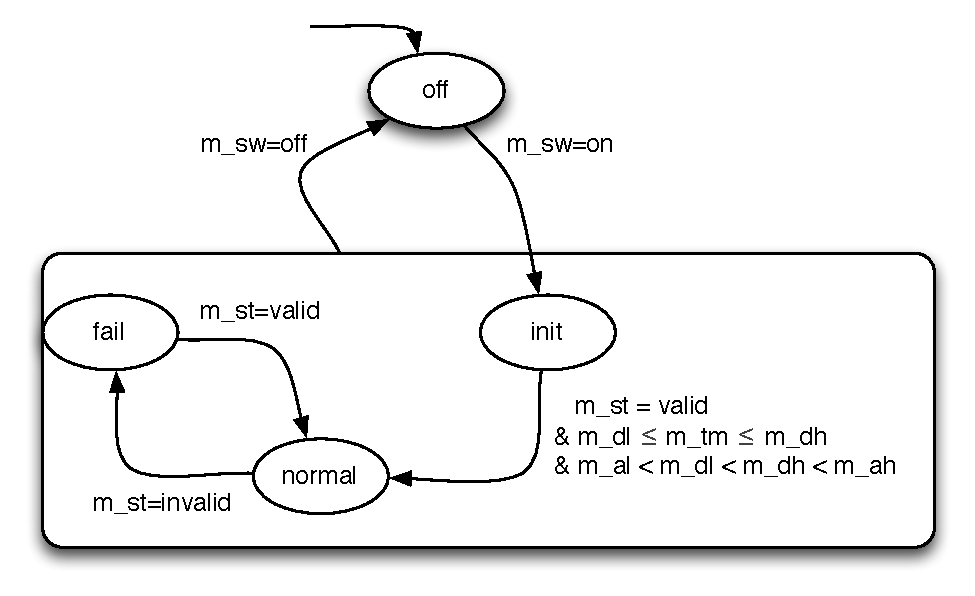
\includegraphics[width=.9\textwidth]{pics/mode-statechart.pdf}
\end{center}
\end{mdframed}
\caption{Statechart for the modes variable \cv{md}}
\label{fig:sc}
\end{figure}

\subsection{Using Everyday Language}
We have stressed mathematically precise function tables and checking them for completeness and disjointness using PVS. However, there is also room for the use of informal English to describe requirements.

Everyday language is (most of the time) the only medium that users and developers share. Everyone
can immediately understand requirements so written; therefore you might think
writing in plain language would be the ideal way to define user needs. 

But simple
text isn't good at showing how different user needs fit together. After all, you
want to make a system, not a mass of unrelated functions. So, you need to make
a structure that will organize the requirements.

The structure must give readers insight into the text. A good structure shows the
requirements at different levels of detail and allows readers to focus on one
section at a time. The users have to understand and dominate the user
requirements, whoever wrote them. A combination of textual requirements and a
scenario-like structure of section headings is very effective. This can be
supplemented if you use simple diagrams.

\subsection{Criteria for good requirements}

Section 3 of \cite{telelogic} contains criteria for good requirement descriptions such as:

\begin{mylist}
\item Is it correct? (does it capture a real user need; does it ask for something possible, do-able, legal)
\item Is it complete? (a complete sentence)
\item Is it clear? (unambiguous and not confusing)
\item  Is it consistent? (not in conflict with other requirements)
\item  Is it verifiable? (can we determine that the system meets the requirement?)
\item Is it traceable? (uniquely identified and can be tracked)
\end{mylist}

\subsection{Descriptions must be atomic and numbered}
Section 2 of \cite{telelogic} contains the definition of good requirement descriptions. The main idea is to break the descriptions into numbered atomic sentences for clarity and traceability. 

The system under design (SUD) in this case is a computer \emph{controller} for the Isolette. The first requirement addresses the required modes of the controller.

\reqm{REQ}
{The \emph{controller} shall operate in one of four modes: \emph{off}, \emph{init}, \emph{normal} and \emph{fail}.\\}
{See statechart in Fig.~\ref{fig:sc} for }
\label{R1}



The atomic description is numbered REQ\ref{R1} in the left cell. The description is in the middle cell. This description must be a complete sentence (subject and predicate) that expresses a \emph{testable} user need (in this case for the nurse to understand the modes of the SUD). 

The right hand cell provides further links to other parts of the requirements document such as function tables or use cases (for traceability). For REQ\ref{R1}, the right hand cell provides a link to a UML statechart (Fig.~\ref{fig:sc}) which describes the sequencing of the modes. UML class diagrams, sequence charts and statecharts are often useful in conveying informal information.\footnote{%
You are required to familiarize yourselves with these diagrams.}

\smallskip
\begin{mdframed}
System modes are distinct discrete behaviours of the system externally \emph{visible} to the users of the system.
\end{mdframed}

In our case, the system modes will be explicitly displayed to nurses operating the Isolette. The nurse will only place a baby in the Isolette in the normal mode. An alarm is activated in the fail mode (see REQ\ref{R3}).\footnote{%
We have deviated from \cite{REMH}. In \cite{REMH}, once the system is in the failed mode, the only way for it to re-enter the normal mode is for the nurse to turn the Isolette off and then on. In or case we raise an alarm in the failed mode, but return to normal if the error condition disappears. The function tables will describe all these changes precisely and in detail.}
Given that the modes of the controller are visible in the ecosystem, the modes are not implementation detail---and may thus appear in the requirements document.

Identification of the major system modes is helpful when writing the detailed system requirements. Initially, it may not be clear if all the system modes have been identified or if all the modes listed are actually needed. The usefulness of any proposed modes will become clear during detailed system requirements specification, and the need for any additional modes will become more apparent. 

Since the system modes are so closely related to the externally visible system behaviour, poor system mode design can lead to mode confusion that may cause the operator to become confused about what mode the system is in. This is an important safety concern that has been implicated in several safety critical accidents \cite{REMH}. 

Some of the potential sources of mode confusion include lack of appropriate feedback to the operators, errors in interpreting or entering information in different modes, inconsistent system behaviours in different modes, different operator authority limits in different modes, silent (unannounced) mode transitions, and unintended side effects of mode transitions. Developing systems in which the modes are clearly indicated to the operators, and the system behaviour is consistent, easily anticipated, and understood by the operators, is a challenging task.


\reqm{REQ}
{In the \emph{normal} mode, the temperature controller shall maintain current temperature inside the Isolette within a set temperature range (the \emph{desired} range).\\}
{The \emph{desired} temperature range is $\mv{dl} \upto \mv{dh}$. If the current temperature \mv{tm} is outside this range, the controller shall turn the heater on or off via the controlled variable \mv{hc} to maintain the desired state.\smallskip}
\label{R2}

It is important to provide a rationale for each E/R-description.  For REQ\ref{R2}, we have:

\smallskip
\noindent \textbf{Rationale}: The \emph{desired temperature range} will be set by the nurse to the desired range based on the infant's weight and health. The controller shall maintain the current temperature within this range under normal operation.

Safety critical requirements such as REQ\ref{R2} emerge from a hazard analysis that must be performed by the safety engineers. The following relevant hazard was identified through the safety assessment process:
\begin{mylist}
\item \textbf{H1}: Prolonged exposure of Infant to unsafe heat or cold;
\item \emph{Classification}: catastrophic;
\item \emph{Probability}: $<10^{-9}$ per hour of operation.
\end{mylist}

\noindent To ensure that probability of hazard H1 is $10^{-9}$ per hour of operation, the following derived safety requirement shall apply to the Isolette controller: 

\reqm{REQ}
{In \emph{normal} mode, the controller shall activate an alarm whenever 

\begin{mylist}
\item the current temperature falls outside the \emph{alarm} temperature range (either through temperature fluctuation or a change in the alarm range by an operator), or
\item a failure is signalled in any of the input devices (temperature sensor and operator settings).
\end{mylist}~}
{The alarm temperature range is $\mv{al}\upto\mv{ah}$.

Monitored variable \mv{st} 
%in Table~\ref{fig:mv} 
shows ``invalid'' when any of the input signals fail.}
\label{R3}


\reqm{REQ}
{Once the alarm is activated, it becomes deactivated in one of two ways:
\begin{mylist}
\item The nurse turns off the Isolette;
\item The alarm has lasted for 10 seconds, and after 10 seconds or more the alarm conditions are removed.
\end{mylist}~\\}
{\hl{Refer to the relevant tables of monitored and/or controlled variables and function tables.}}
\label{R4}

The following is an E-description because it does not describe a function that the SUD might enforce; rather, it is a constraint imposed by the environment over which the SUD has no control. 
\reqm{ENV}
{The current temperature received from the sensor is a a real number in the range $68.0$ to $105.0 \degree{F}$.\\}
{\hl{Refer to the relevant tables of monitored and/or controlled variables and function tables.}}
\label{E1}

This is important information. The computer controller need not deal with temperatures above or below the stated range. We may also use ENV\ref{E1} as an assumption  when we provide function tables--which may omit ranges that will not occur (in completeness and disjointness analysis). Here is another example of an E-description:

\reqm{ENV}
{The desired and alarm temperatures received from the operator are all in increments of $1 \degree{F}$.\\}
{\hl{Refer to the relevant tables of monitored and/or controlled variables and function tables.}}
\label{E2}

As before, it is important to provide a rationale for each E and R description. For example, for ENV\ref{E2}, the rationale is: Marketing studies have shown that customers prefer to set temperatures in 1 degree increments. A resolution $1\degree{F}$ is sufficient to be consistent with the functional and performance requirements specified in the rest of the document. 

We can mix the atomic descriptions with informal text showing rationale as we have done here. By placing the atomic E/R-descriptions in a box, we allow them to stand out from the informal text. The same procedure is followed in mathematical text books where theorems and definitions are placed in a box or a special numbered environment for easy reference.

\subsection{Real-time and the held-for operator}

\begin{figure}[htbp]
\begin{center}
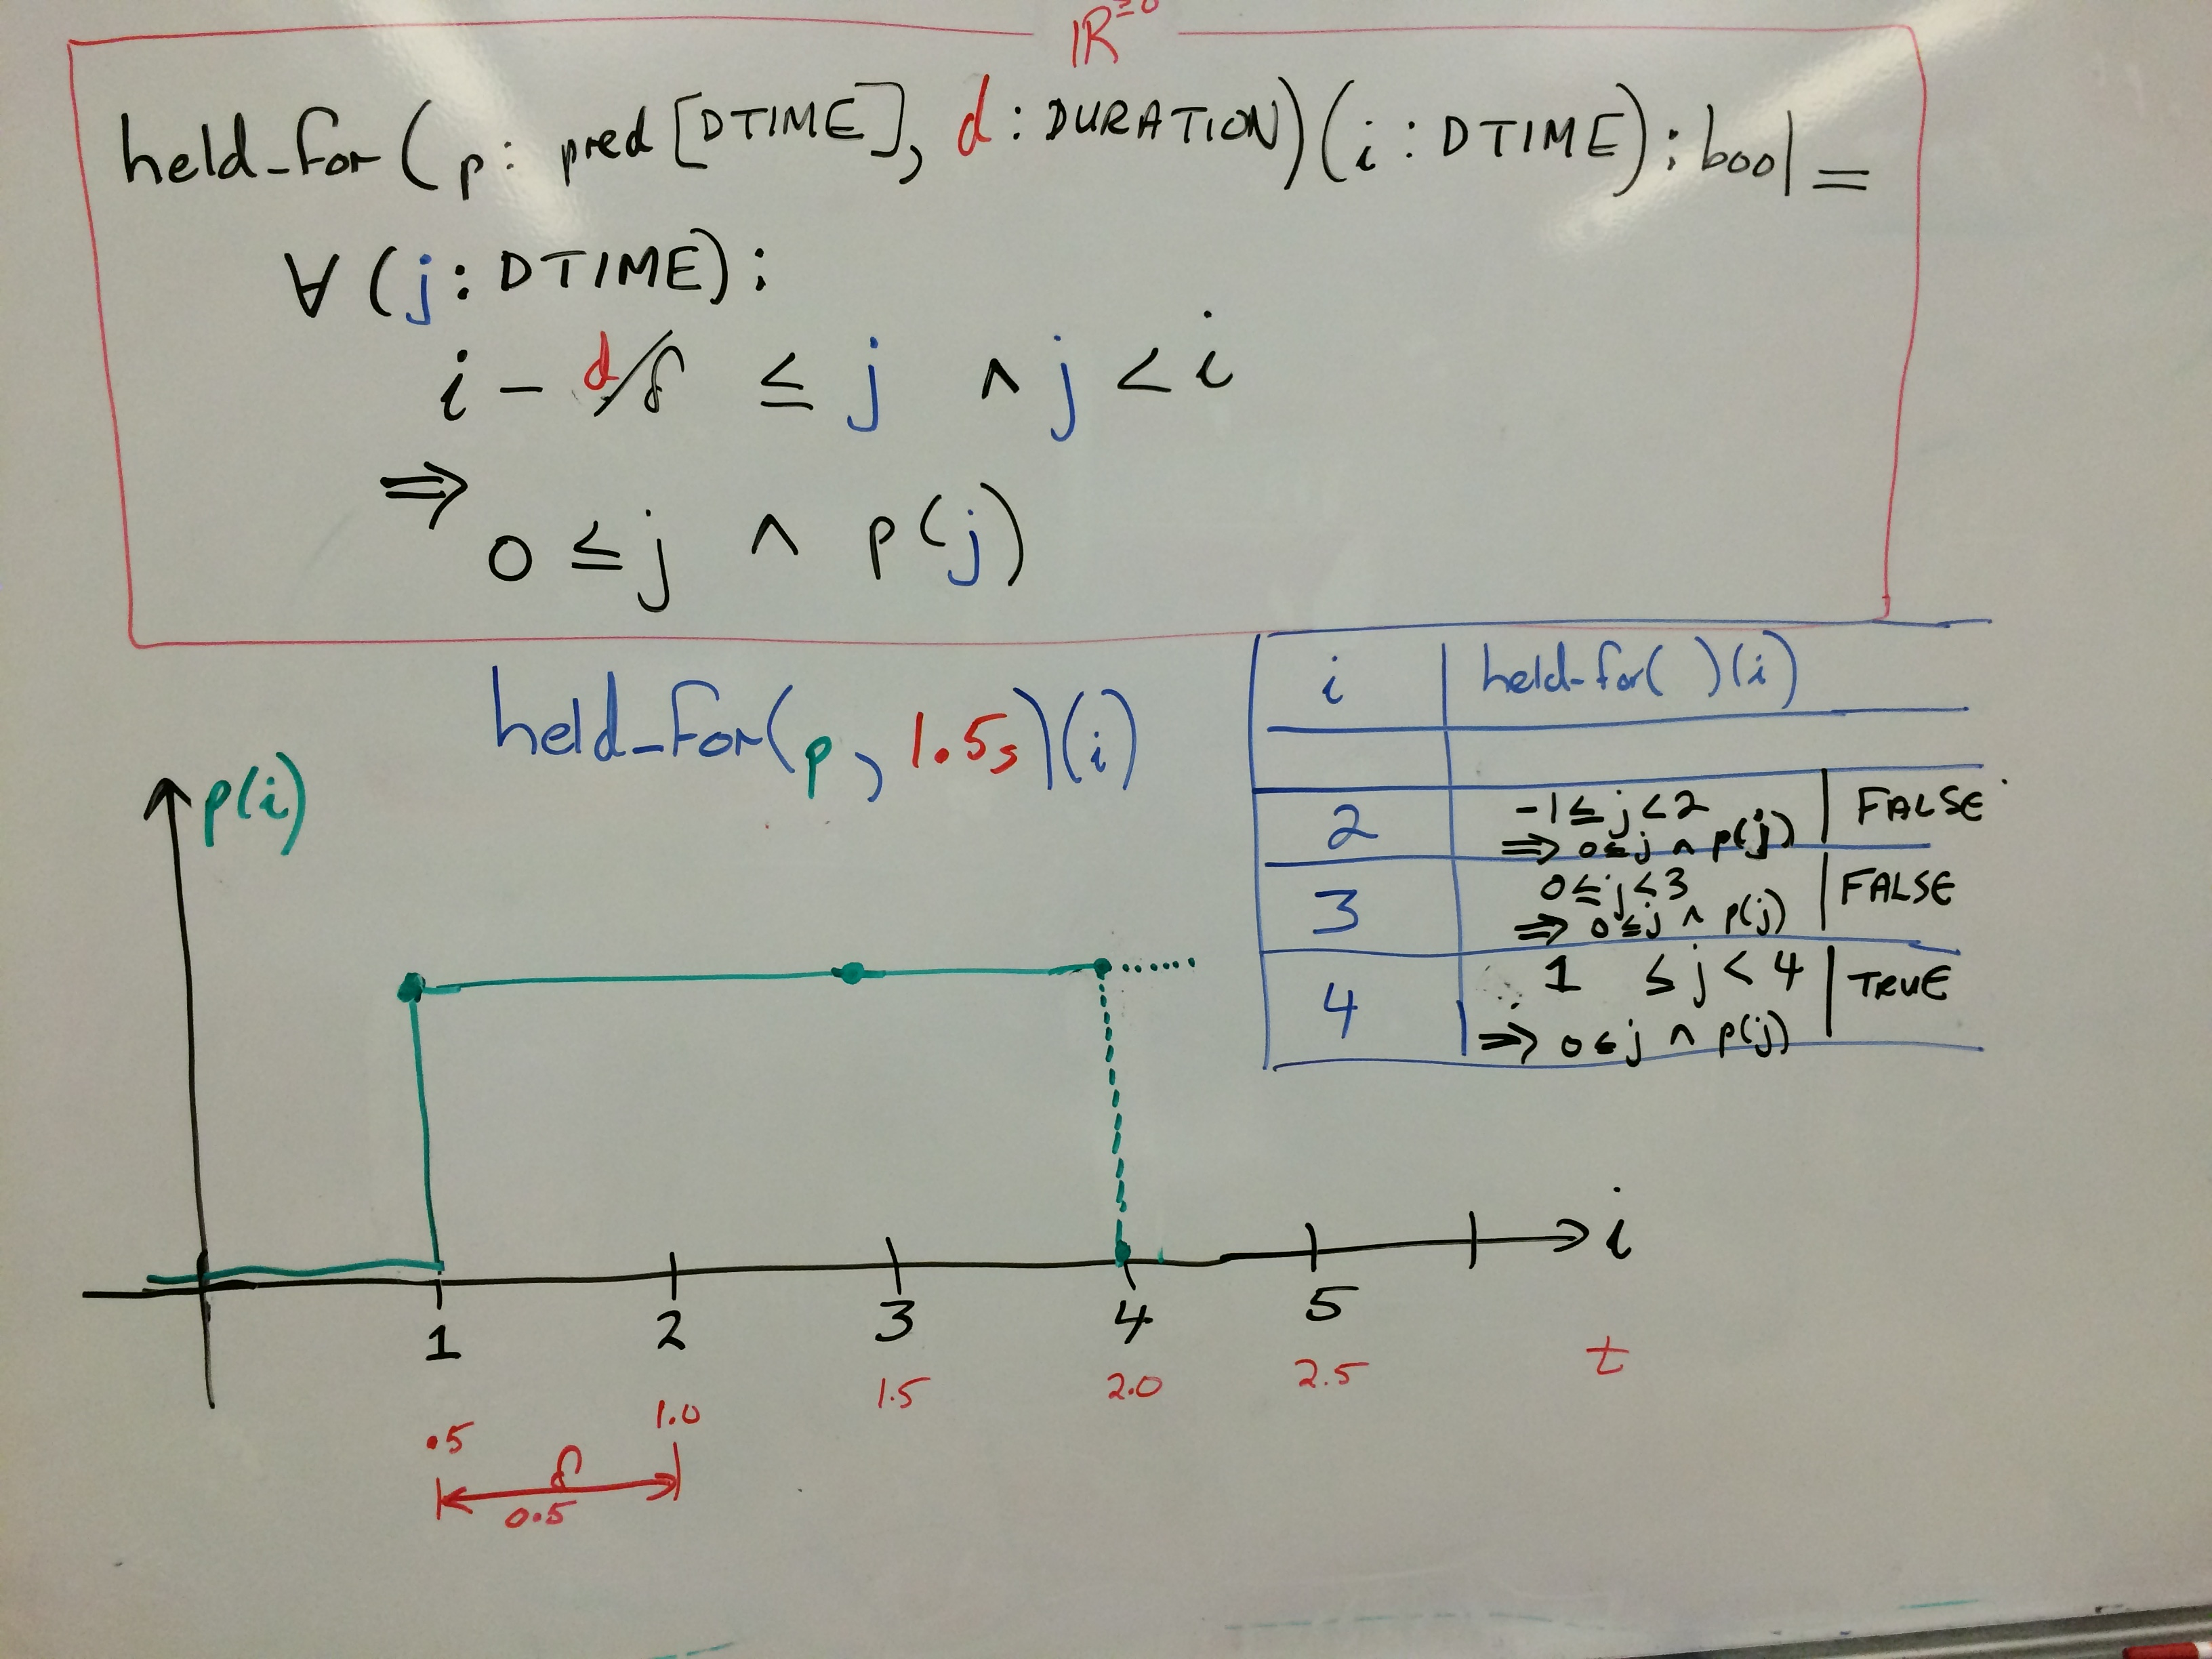
\includegraphics[width=\textwidth]{pics/held-for.jpg}
\caption{Using the held\_for operator: $held\_for(p,1.5s)(i)$}
\label{fig:held}
\end{center}
\end{figure}

Given that REQ\ref{R4} provides a time (10 seconds) for the persistence of the alarm alert, appropriate attention must be paid to timing issues. Review the course slides on timing resolutions (TR) and response allowances (RA). See also \cite{WLH05} (also in the course SVN).\footnote{%
The discussion of tolerances in the \cite{WLH05}  is out of scope for this assignment. However, the rest of the article provides an nice review of timing resolutions and response allowances.}

Reference \cite{WLH05} provides a useful operator---the \emph{held-for} operator---that may be used in function tables using  our $\delta$ time theory (see Appendix~\ref{sec:time} for the complete theory):

\begin{pvs}
  DURATION: TYPE = nnreal
  held_for(p: pred[DTIME], d: DURATION)(i:DTIME): bool =
    (FORALL (j: DTIME): 
    i - (d / delta) <= j AND j < i IMPLIES 0 <= j AND p(j))
\end{pvs}


As an example, consider the predicate $p: [DTIME \tfun \Bl]$ shown in the graph of Fig.~\ref{fig:held} (in green) where the timing resolution is $\delta = 0.5s$. The predicate $held\_for(p,1.5)(i)$ holds at $i=4$ because in the immediately preceding three digital time units ($j \in 1\upto3$) spanning 1.5 seconds, $p(j)$ holds true.\footnote{%
At $j=4$ the signal might stay true or go false.}

However, at instant $i=3$ and below, the held-for predicate is false. 
The left operand ($0\leq j$) of the consequent 
$0 \leq j \land p(j)$ in the held-for definition ensure that the held-for is always false at instants $i=0$ and $i=1$.

The PVS specification in Fig.~\ref{fig:hft}  illustrates a use case for the held-for operator in a function table.

\begin{figure}
\begin{pvs}
alert: THEORY
BEGIN
  delta: posreal = 1 % TR = 1 seconds
  IMPORTING Time[delta]
  
  signal: VAR [DTIME -> bool] % input
  alert: VAR [DTIME -> bool]  % output

  response(signal)(alert)(i:DTIME): bool =
    COND
        i = 0 -> NOT alert(i) 
      , i > 0 -> 
        COND
             signal(i) 
          -> alert(i)=TRUE,
             NOT signal(i) AND held_for(alert,3)(i) 
          -> alert(i) = FALSE,        
             ELSE 
          -> alert(i) = alert(i-1)
          ENDCOND
   ENDCOND

  check1: CONJECTURE
        signal(0) = FALSE
    AND signal(1) = TRUE
    AND response(signal)(alert)(0)
    AND response(signal)(alert)(1)
    AND response(signal)(alert)(2)
    AND response(signal)(alert)(3)
    =>
      alert(1) AND alert(2) AND alert(3)
      
END alert
\end{pvs}
\caption{Example of a function table using the held-for operator}
\label{fig:hft}
\end{figure}


\subsection{Pitfalls to avoid}

See Sections A and F of \cite{telelogic} for pitfalls to avoid.

For example, don't try to fit multiple needs into a single atomic description.
R-descriptions which contain conjunctions (words that join sentences together)
are dangerous. Problems arise when readers try to puzzle out which part applies,
especially if the different clauses seem to conflict, or if the individual parts apply
separately. Dangerous conjunctions include and, or, with, also.

\smallskip
\textbf{Example of a Bad description}:
\emph{The battery low warning lamp shall light up when the voltage drops below 3.6
Volts, and the current workspace or input data shall be saved.}

\bigskip
Don't ramble. Long rambling sentences, especially when combined with arcane language,
references to unreachable documents, and other defects of writing, quickly lead
to confusion and error.

\textbf{Example of a Bad description}:
\emph{Provided that the designated input signals from the specified devices are received
in the correct order where the system is able to differentiate the designators, the
output signal shall comply with the required framework of section 3.1.5 to
indicate the desired input state.}

\bigskip
Refrain from designing the system. Requirements specify the design envelope, and if we supply too much detail we
start to design the system. Going too far is tempting for designers, especially
when they come to their favourite bits. Danger signs include names of
components, materials, software objects/procedures, and database fields.

\textbf{Example of a Bad description}:
T\emph{he antenna shall be capable of receiving FM signals, using a copper core with
nylon covering and a waterproof hardened rubber shield.}

Specifying design rather than actual need increases the cost of systems by placing
needless constraints on development and manufacture. Often knowing why is
much better than knowing what.

For Assignment 1, only the the parts \hl{highlighted in yellow}, in the sequel,  are to be done.

\section{Changes in the specifications from  REMH \cite{REMH}}

For the Assignment,  for simplicity, clarity and safety---there are some changes in the specification of the Isolette,  from those descriptions provided in \cite{REMH}. Some of the changes include:

\begin{mylist}
\item The statechart for the modes is in Fig.~\ref{fig:sc}.
\item The monitored and controlled variables of the SUD are provided in the assignment template.\footnote{\texttt{a1-Isolette.pdf}.}
\item The R-description REQ\ref{R4} requires that the alarm is held for 10 seconds.
\item See below.
\end{mylist}

\subsection{Constraints on the desired/alarmed inputs}

The SUD is the computer \emph{controller} to regulate temperature. Everything else, including the Operator Interface is in the exosystem (i.e. in the environment of the controller).  The Appendix-A specification of the Isolette \cite[pA-11]{REMH} states:

\begin{quote}
EA-OI-4: The Lower Alarm Temperature will always be less than or equal to the Lower Desired Temperature of $-1\degree{F}$.

\textbf{Rationale}: If the Lower Alarm Temperature is greater than or equal to the Lower Desired Temperature, the Alarm could be activated while the Current Temperature is still in the Desired Temperature Range.

EA-OI-6: The Lower Desired Temperature will always be less than or equal to the Upper Desired Temperature of  $-1\degree{F}$.
\end{quote}

The above constraints are stated in \cite{REMH}  as E-descriptions (i.e. environmental descriptions) on the Isolette. What EA-OI-4, for example, implies is that the \emph{controller} can assume that \mv{al} is always less than \mv{dl}  (like a precondition). Who ensures that this constraint is satisfied? Apparently there is a device in the exosystem called the Operator Interface whose function is to ensure that this constraint is obeyed.

However, for the purposes of this Assignment, we may not rely on these constraints on the monitored variables in specifying the computer controller (the SUD). Thus the controller shall generate an alarm if there is a problem with the relationship between the desired and alarmed inputs. \textbf{Rationale}: This provides an extra check on the alarm and desired inputs, given the safety critical nature of the Isolette.

Thus, the only constraints that we may assume are on the types and ranges of the desired and alarm inputs (as stated in Appendix A of REMH). For example, we may assume that desired lower temperature range of \mv{d} is $97\upto 99$ and the lower alarm temperature range is always $93\upto 98$.

\subsection{Alarm Off Hysteresis and Displayed Temperature}

\begin{figure}[htbp]
\begin{mdframed}
\begin{center}
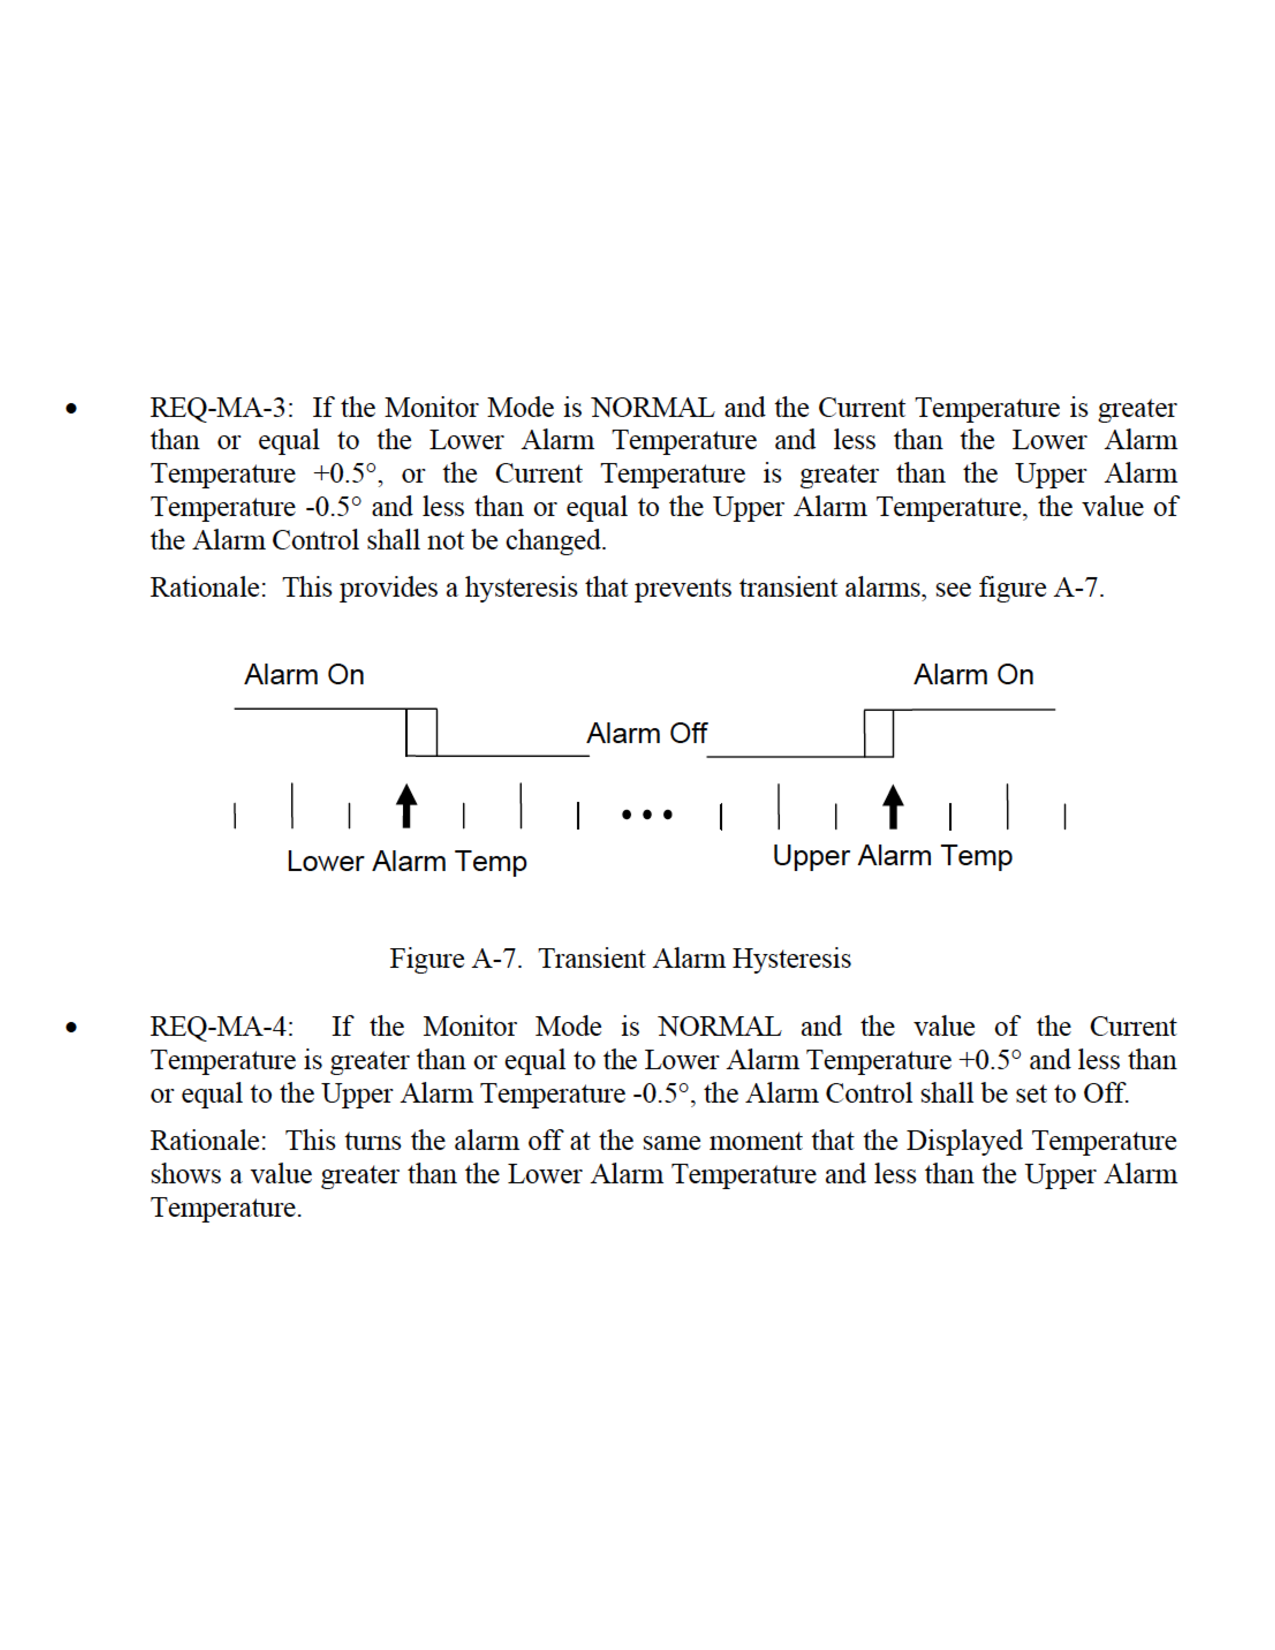
\includegraphics[width=.9\textwidth]{pics/hysteresis.pdf}
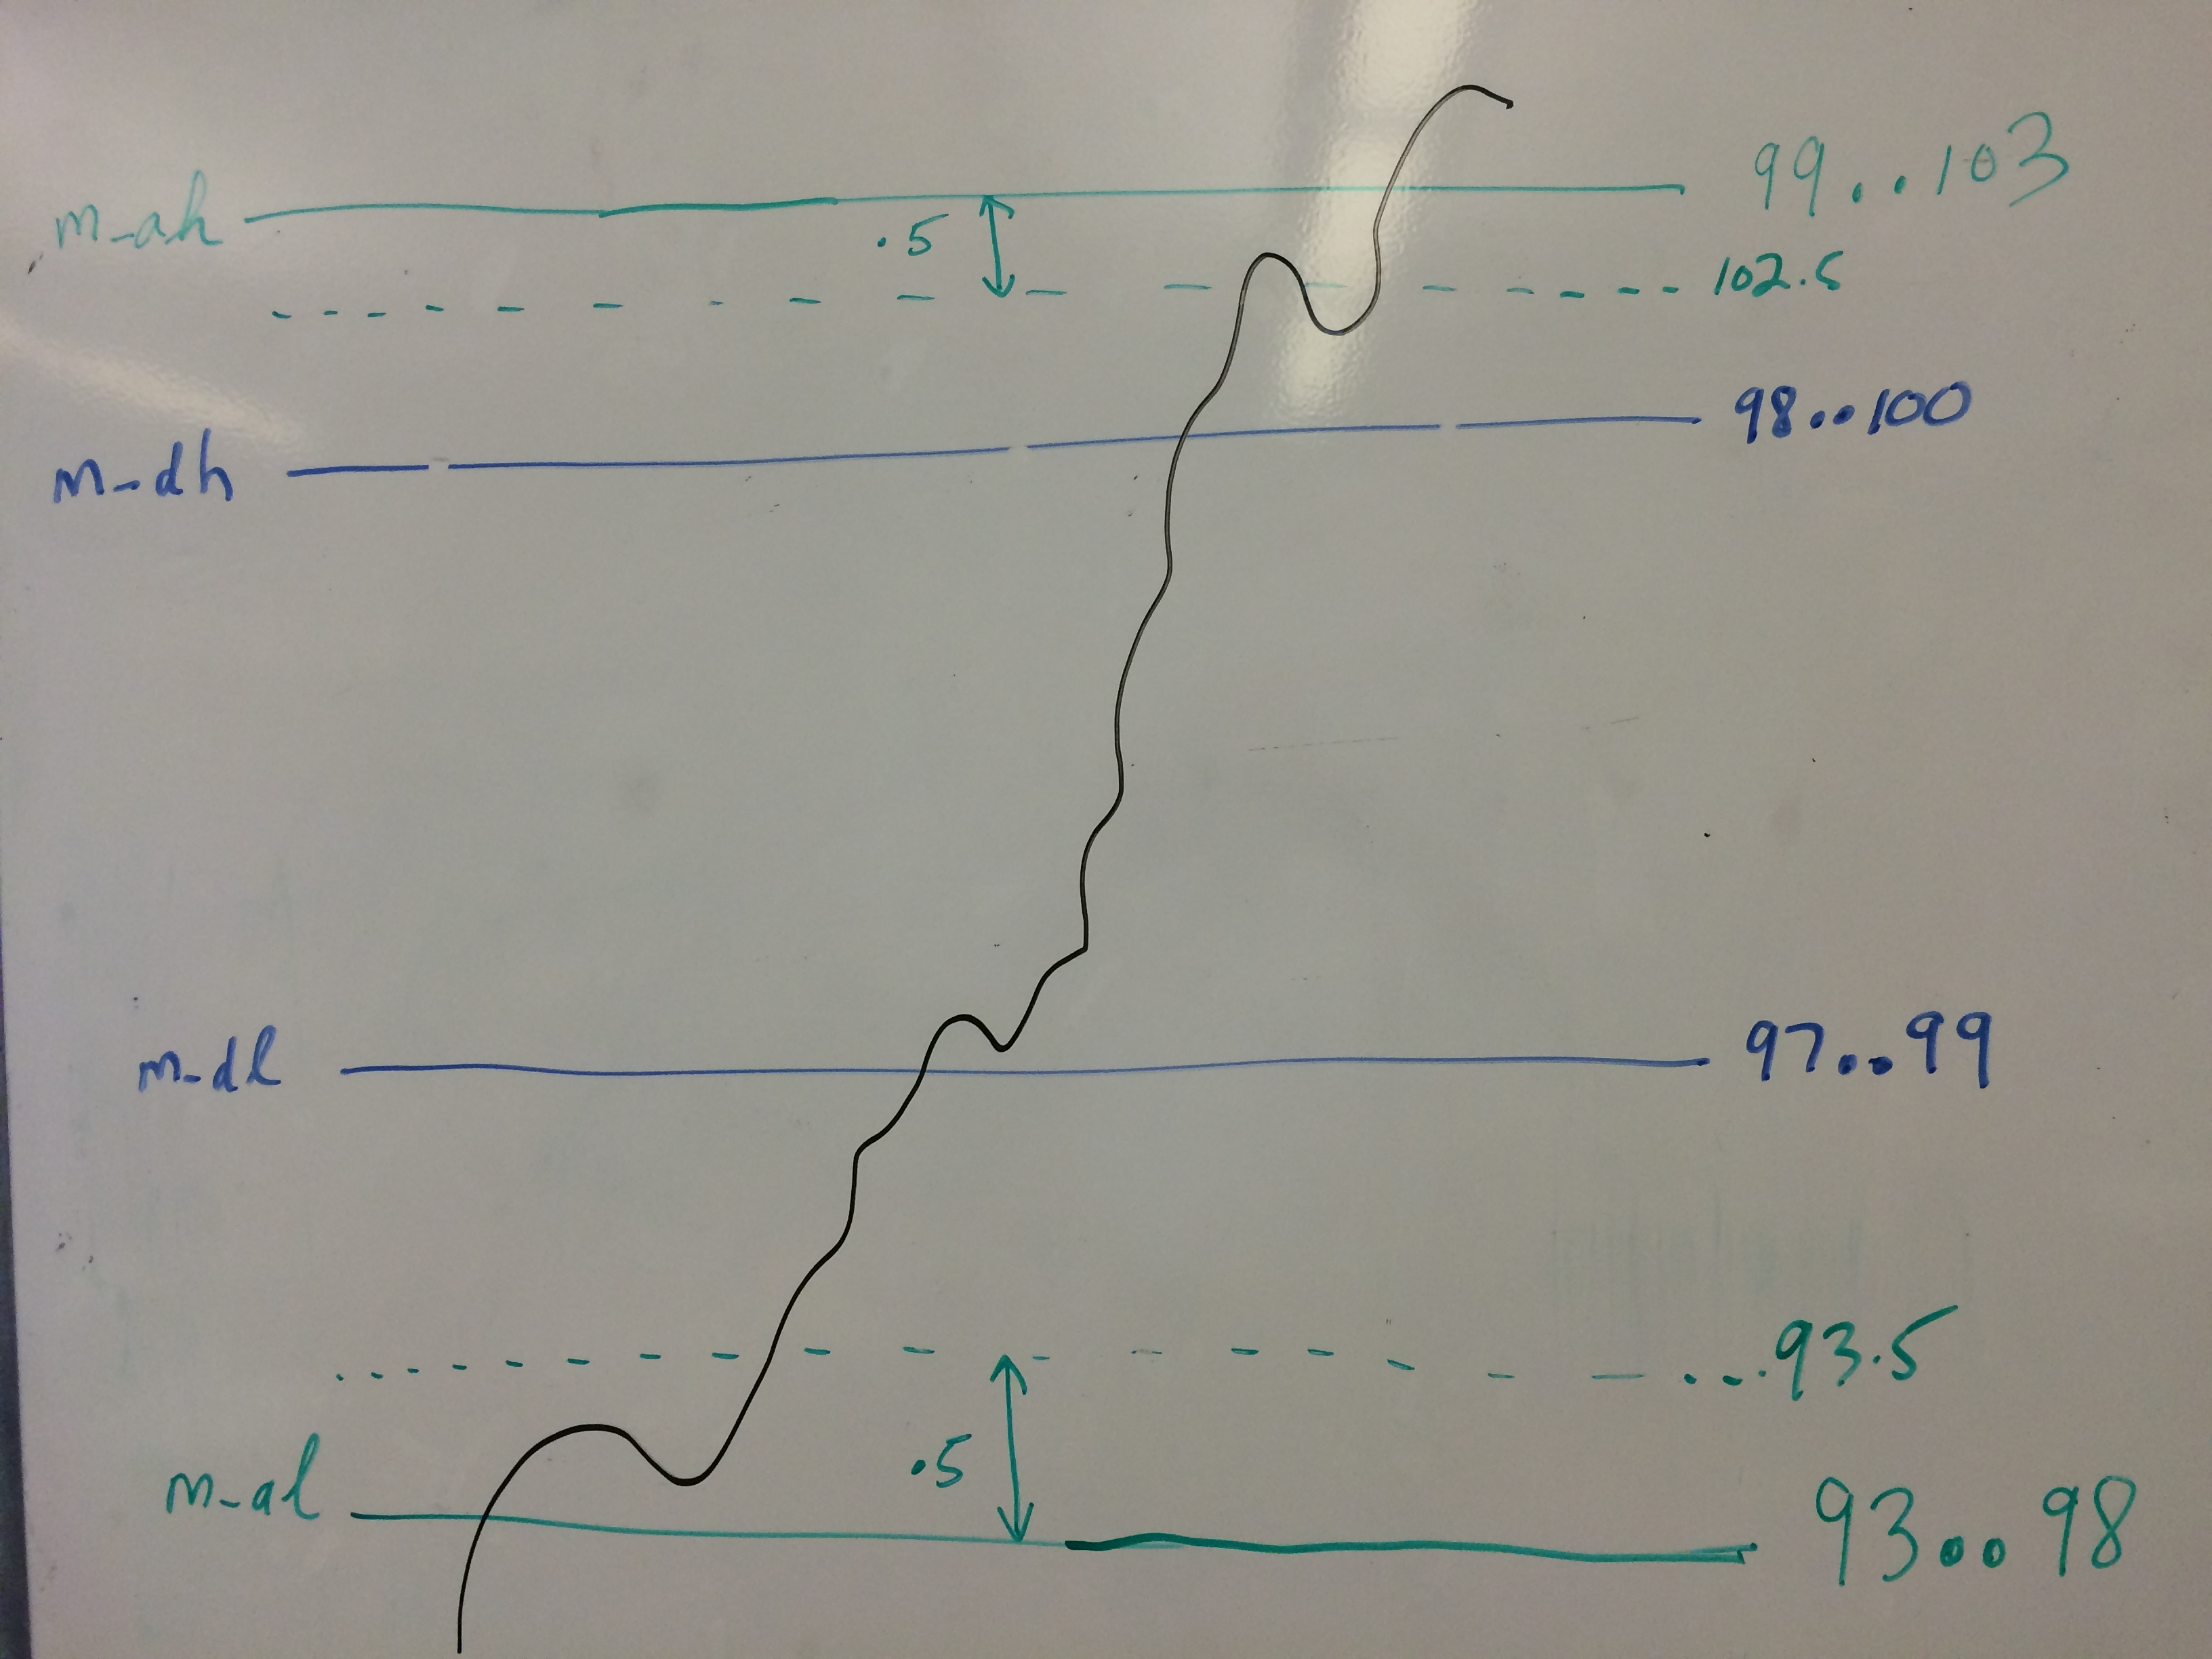
\includegraphics[width=.9\textwidth]{pics/hysteresis.jpg}
\end{center}
\end{mdframed}
\caption{Hysteresis requirement for management of Alarm Off in \cite{REMH}}
\label{fig:hys}
\end{figure}

There appears to be an inconsistency in \cite{REMH} in the specifiaction for turning the alarm off. A  snippet of the specification is shown in Fig.~\ref{fig:hys}. If we translate REQ-MA-3 to mathematical notation we find that the no change hysteresis band is defined by:

\begin{align}
\textrm{no-change hysteresis band for low alarm}: \quad &\label{eq:1}
\mv{al} \leq \mv{tm} < \mv{al}+ 0.5\\
\textrm{no-change hysteresis band for high alarm}: \quad &\label{eq:2}
\mv{ah} -0.5 < \mv{tm} \leq \mv{ah} 
\end{align}

\noindent We assume, for simplicity, that standard engineering rounding will be used, i.e.

\begin{align}
\cv{td} = \lfloor \mv{tm} + 0.5\rfloor \label{eq:rd}
\end{align}

\noindent Thus for example, assume that the high alarm is on when the current temperature is above 103 and then decreases into the hysteresis band (NC). When the temperature further decreases to 102.5 which is outside of the hysteresis band according to (\ref{eq:2}), the alarm is turned off. However, standard rounding means that $\cv{td}$ displays 103---meaning the alarm should still be on. This inconsistency will be a source of confusion for the nurses.

We thus need to change  (\ref{eq:2}) to:

\begin{align}
\textrm{no-change hysteresis band for high alarm}: \quad &\label{eq:3}
\mv{ah} -0.5 \leq \mv{tm} \leq \mv{ah} 
\end{align}

\noindent The proof that (\ref{eq:1}) and (\ref{eq:3}) are consistent with rounding scheme (\ref{eq:rd}) is provided in Fig.~\ref{fig:proof}.

\begin{figure}[htbp]

\begin{mdframed}\small
\begin{align}
\cv{td} = \lfloor \mv{tm} + 0.5\rfloor \tag{0}
\end{align}
\begin{align}
\textrm{no-change hysteresis band for low alarm}: 
\mv{al} \leq \mv{tm} < \mv{al}+ 0.5 \tag{1}\\
\textrm{no-change hysteresis band for high alarm}: 
\mv{ah} -0.5 \leq \mv{tm} \leq \mv{ah} \tag{4}
\end{align}

The condition that turns the alarm off (if the alarm had been on for temperatures above $\mv{ah}$) is $\mv{tm} < \mv{ah} -0.5$, which is 
the negation of the left inequality of (4). The rationale behind REQ-MA-4 tells us that the moment when the alarm is turned off---the displayed temperature is strictly below the upper alarm temperature  \mv{ah}. Hence the first equivalence below. Likewise for the second equivalence.
\bigskip
\begin{center}
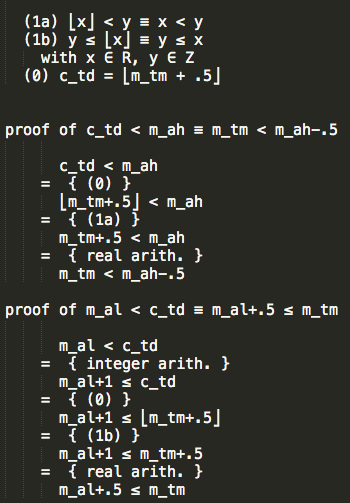
\includegraphics[width=.5\textwidth]{pics/hysteresis-proof.png}
\end{center}
\end{mdframed}
\caption{Proof that hysteresis bands (\ref{eq:1}), (\ref{eq:3}) are consistent with rounding scheme (\ref{eq:rd}) }
\label{fig:proof}
\end{figure}

%%%%%%%%%%%%%%%%%%%%%
\section{Function Tables Require Non-circular Data Flow}

When writing function tables that depend upon each other, it is important to avoid circularity in the data flow.

%%%%%%%%%%%%%%%%%%%%%%%%%%%%%%%%
\begin{figure}[htbp]
\begin{mdframed}
\begin{center}

Inputs $m_1,m_2$, states $s_1, s_2$ and outputs $c_1,c_2$

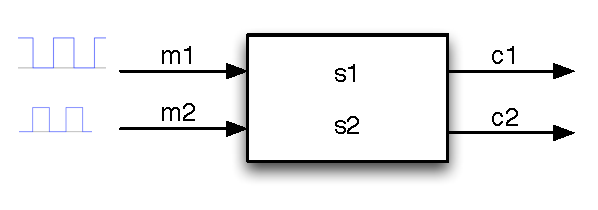
\includegraphics[width=.8\textwidth]{pics/dataflow.pdf} 
\end{center}
\end{mdframed}

\caption{Specification of a Function Block}
\label{fig:fb}
\end{figure}
%%%%%%%%%%%%%%%%%%%%%%%%%%%%%%

Consider the two inputs $m_1$ and $m_2$ (the monitored variables) in Fig.~\ref{fig:fb} which are square waves coming from the ecosystem. The goal is that (a) the output $c_1$ (a controlled variable) shall provide a count of the total number of times the the inputs change from 0 to 1 and (b) $c_2$ shall provide a count of the average number of transitions over time.   

It is convenient to introduce internal states $s_1$ and $s_2$ to specify the counts of up-edges coming into the system as shown in Fig~\ref{tbl:state}. Output $c_1$ is defined in terms of the internal states, and output $c_2$ in terms of $c_1$.

\begin{figure}[h]
\centering 
\begin{tabular}{ll|l|}
\cline{3-3}
\multicolumn{2}{l}{}                                                                   & \cellcolor[HTML]{EFEFEF}$s_1(i):\nat$ \\ \hline
\multicolumn{2}{|l|}{$i=0$}                                                            & 0                                \\ \hline
\multicolumn{1}{|l|}{}                          & $m_1(\im{1}) = 0 \1\land m_1(i) = 1$ & $s_1(\im{1}) + 1$                \\ \cline{2-3} 
\multicolumn{1}{|l|}{\multirow{-2}{*}{$i > 0$}} & $m_1(\im{1}) = 1 \1\lor m_1(i) = 0$  & NC                               \\ \hline
\end{tabular}
\quad
\begin{tabular}{l|l|}
\cline{2-2}
                           & $c_1(i):\nat$ \\ \hline
\multicolumn{1}{|l|}{true} & $s_1(i) + s_2(i)$       \\ \hline
\end{tabular}

\bigskip
\begin{tabular}{ll|l|}
\cline{3-3}
\multicolumn{2}{l}{}                                                                   & \cellcolor[HTML]{EFEFEF}$s_2(i):\nat$ \\ \hline
\multicolumn{2}{|l|}{$i=0$}                                                            & 0                                \\ \hline
\multicolumn{1}{|l|}{}                          & $m_2(\im{1}) = 0 \1\land m_2(i) = 1$ & $s_2(\im{1}) + 1$                \\ \cline{2-3} 
\multicolumn{1}{|l|}{\multirow{-2}{*}{$i > 0$}} & $m_2(\im{1}) = 1 \1\lor m_2(i) = 0$  & NC                               \\ \hline
\end{tabular}
\quad
\begin{tabular}{l|l|}
\cline{2-2}
                            & $c_2(i)\Rl$   \\ \hline
\multicolumn{1}{|l|}{$i=0$} & 0          \\ \hline
\multicolumn{1}{|l|}{$i>0$} & $c_1(i)/i$ \\ \hline
\end{tabular}

\caption{Outputs $c_1$ and $c_2$ defined in terms of internal states $s_1, s_2$}
\label{tbl:state} 
\end{figure}

%%%%%%%%%
\begin{figure}[!t]
\begin{mdframed}
\begin{center}
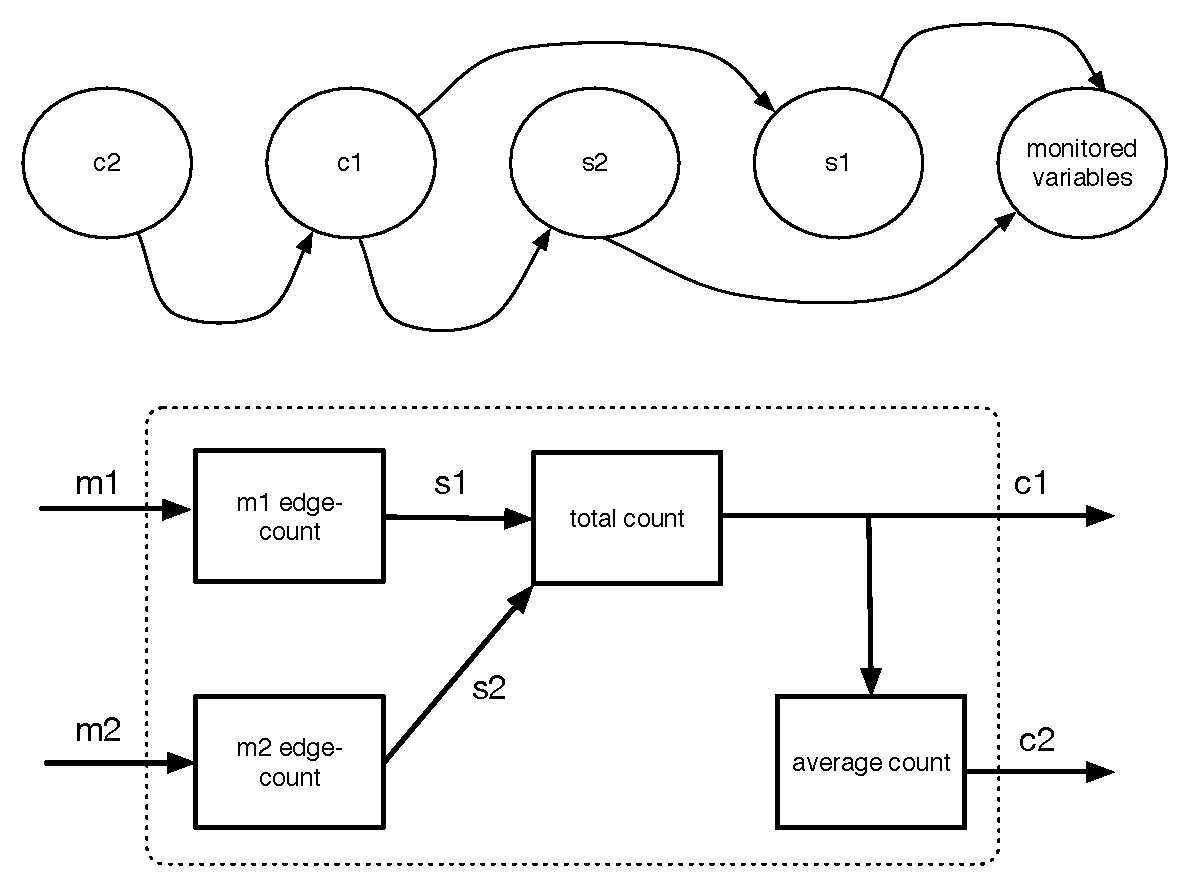
\includegraphics[width=.9\textwidth]{pics/topological.pdf}
\end{center}

Let $x(j\upto k)$ stand for values of variable $x$ at instants $j$ to $k$, i.e.\\
$x(j), x(j+1), x(j+2),\ldots,x(k)$. Then the data-flow is non-circular provided:
\small
\begin{align}
c_2(i) &= f_1(c_2(0 \upto \im{1}), c_1(0\upto i), s_2(0\upto i), s_1(0\upto i), m_2(0\upto i), m_1(0\upto i))\\\label{eqn:coherent}
c_1(i) &= f_2(c_2(0\upto \im{1}), c_1(0\upto \im{1}), s_2(0\upto i), s_1(0\upto i), m_2(0\upto i), m_1(0\upto i))\\
s_2(i) &= f_3(c_2(0\upto \im{1}), c_1(0\upto \im{1}), s_2(0\upto \im{1}), s_1(0\upto i), m_2(0\upto i), m_1(0\upto i))\\
s_1(i) &= f_4(c_2(0\upto \im{1}), c_1(0\upto \im{1}), s_2(0\upto \im{1}), s_1(0\upto \im{1}), m_2(0\upto i), m_1(0\upto i))
\end{align}
\normalsize
The monitored variables, being read-only, can always be referred to at any current or past instant. The control and state variables can also be written to---so it is with these that we have to exercise caution to ensure that the data-flow is valid.
\end{mdframed}
\caption{Topological sort order: No circularities in the function tables in Fig.~\ref{tbl:state}}
\label{fig:topological}
\end{figure}
%%%%%%%%%%%

\subsection{Circularity and data-flow}

In Fig~\ref{tbl:state}, $c_1(i) = s_1(i) + s_2(i)$. Is there any circularity in the data flow? As it happens, this specification is valid. Fig.~\ref{fig:topological} provides conditions under which non-circular data-flow is preserved. Function tables must be written in a fashion that avoids circularities.

Consider, for example, a different definition: $c_1(i) = c_1(i) + 1$. Here there is obviously a problem because the expression reduces to $0 = 1$, which is false. One cannot define $c_1(i)$ in terms of itself!

What about $c(i) = c(\im{1}) + 1$? That is ok, because c(\im{1})  is the value of $c(i)$ in the past. We are not asserting something that is incoherent. Rather, we are asserting that value of $c$ at instant $i$ is one more than its value in the previous instant. This is why the definitions of $s_1$ and $s_2$ are also valid as they only refer to their values in the past. 


In Fig.~\ref{tbl:state}, $c_2(i) = c_1(i)/i$ (for positive time instances). Can we define $c_2(i)$---a controlled variable---in terms of another controlled variable? Yes, provided there is no circularity. The following is circular and thus incoherent:

\bigskip
\begin{center}
\fbox{\begin{minipage}{0.4\textwidth}
\begin{align*}
\textrm{Circular:}\\
&c_2(i) = c_1(i) + 1\\
&c_1(i) = c_2(i) + 1
\end{align*}
\end{minipage}}
\end{center}
\bigskip

\noindent which asserts that $0=2$.

So what are the general rules to avoid circular data flows. The ability to place the variable dependencies in topological order will ensure that there are no circular data flows. The dependency graph for the function tables in  Fig.~\ref{tbl:state} is in Fig.~\ref{fig:topological}. Since there is no circularity in the dependency graph, the function tables are valid. See equation (\ref{eqn:coherent}) in  Fig.~\ref{fig:topological} for the general constraints on writing connected function tables (modules).

\subsection{Using abstract state variables}
It is not necessary to use internal state to describe the system. It is possible to write the control variables in the current instant purely in terms of the monitored variables at the current instant and earlier. For example, using the counting quantifier \#, we may write:

\begin{align*}
c_1(i) &= (\#j \in 1\upto i: m_1(j-1) = 0 \1\land  m_1(j)=1)\\
 & \qquad + (\#j \in 1\upto i: m_2(j-1) = 0 \1 \land m_2(j)=1)
\end{align*}
















%%%%%%%%%%%%%%%%%%%%%%%%%%%%%%%%%%%%%
\bibliographystyle{plain}
\bibliography{ref}

\appendix 

\section{PVS Time theory for held-for operator}\label{sec:time}

\begin{pvs}
Time[delta: posreal]  : THEORY
BEGIN
  % digital time
  DTIME : TYPE = nat
  init(i : DTIME) : bool = i = 0 

  % pseudo, digitized real time   
  RTIME : TYPE = {t : nnreal | (EXISTS (i : DTIME) : t = i * delta)}

  % actual time
  TIME : TYPE = nnreal

  % Positive DTIME
  POS_DTIME: TYPE = posnat
  
  % conversions
  r2d(t: RTIME): DTIME = t / delta
  d2r(i: DTIME): RTIME = i * delta

  DURATION: TYPE = nnreal
  held_for(p: pred[DTIME], d: DURATION)(i:DTIME): bool =
    (FORALL (j: DTIME): 
    i - (d / delta) <= j AND j < i IMPLIES 0 <= j AND p(j))

END Time
\end{pvs}

\section{Outline of a Precise Requirements Document}

\begin{figure}[htbp]
\begin{mdframed}
\begin{center}
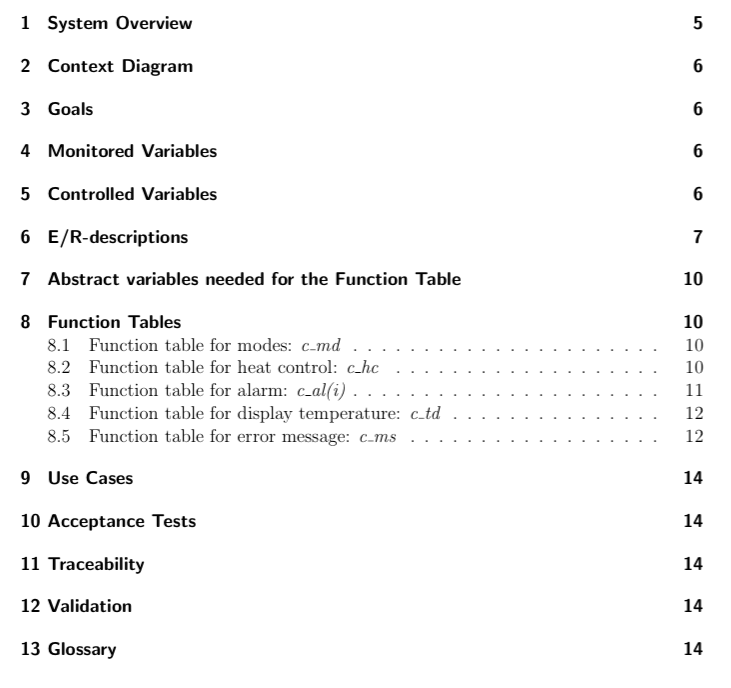
\includegraphics[width=\textwidth]{pics/outline.png}
\end{center}
\end{mdframed}
\end{figure}
\end{document} 